% Generated 2021-02-25 13:56:55 +0530
\subsection{CuttingItem} \label{sec:CuttingItem}


A \block{CuttingItem} is the portion of the tool that physically removes the material from the workpiece by shear deformation.  The Cutting Item can be either a single piece of material attached to the \block{CuttingItem} or it can be one or more separate pieces of material attached to the \block{CuttingItem} using a permanent or removable attachment.  A \block{CuttingItem} can be comprised of one or more cutting edges. \block{CuttingItems} include: replaceable inserts, brazed tips and the cutting portions of solid \block{CuttingTools}.

MTConnect Standard considers \block{CuttingItems} as part of the \block{CuttingTool}.  A \block{CuttingItems} \textbf{MUST NOT} exist in MTConnect unless it is attached to a \block{CuttingTool}.  Some of the measurements, such as \block{FunctionalLength}, \textbf{MUST} be made with reference to the entire \block{CuttingTool} to be meaningful.

\begin{figure}[ht]
  \centering
    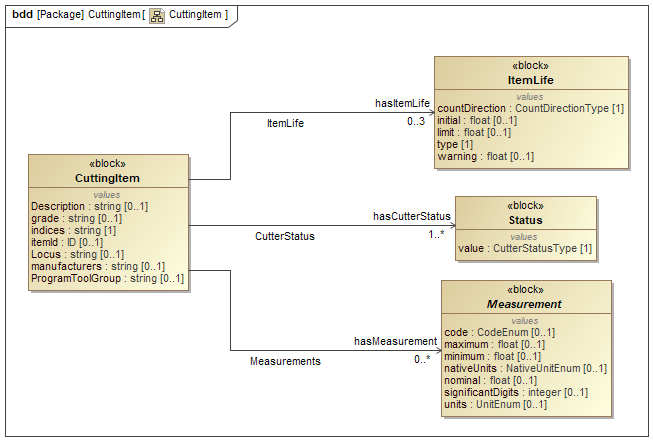
\includegraphics[width=1.0\textwidth]{figures/CuttingItem.png}
  \caption{CuttingItem Diagram}
  \label{fig:CuttingItem Diagram}
\end{figure}

\FloatBarrier


Note: See \sect{CuttingItem Schema Diagrams} for XML schema.


\subsubsection{CuttingItem}




A \block{CuttingItem} is the portion of the tool that physically removes the material from the workpiece by shear deformation.


\paragraph{Attributes of CuttingItem}\mbox{}
\label{sec:Attributes of CuttingItem}

\tbl{Attributes of CuttingItem} lists the attributes of \texttt{CuttingItem}.

\begin{table}[ht]
\centering 
  \caption{Attributes of CuttingItem}
  \label{table:Attributes of CuttingItem}
\tabulinesep=3pt
\begin{tabu} to 6in {|l|l|l|} \everyrow{\hline}
\hline
\rowfont\bfseries {Attribute} & {Type} & {Multiplicity} \\
\tabucline[1.5pt]{}

\property{grade}[CuttingItem] & \texttt{string} & 0..1 \\
\property{indices}[CuttingItem] & \texttt{string} & 1 \\
\property{itemId}[CuttingItem] & \texttt{ID} & 0..1 \\
\property{manufacturers}[CuttingItem] & \texttt{string} & 0..1 \\
\end{tabu}
\end{table}
\FloatBarrier

Descriptions for attributes of \block{CuttingItem}:

\begin{itemize}

\item \property{grade}[CuttingItem] \newline The material composition for this Cutting Item.


\item \property{indices}[CuttingItem] \newline The number or numbers representing the individual Cutting Item or items on the tool.


\item \property{itemId}[CuttingItem] \newline The manufacturer identifier of this Cutting Item.

\item \property{manufacturers}[CuttingItem] \newline The manufacturers of the Cutting Item.

The representation will be a comma(,) delimited list of manufacturer names.
\end{itemize}


\paragraph{Elements of CuttingItem}\mbox{}
\label{sec:Elements of CuttingItem}

\tbl{Elements of CuttingItem} lists the elements of \texttt{CuttingItem}.

\begin{table}[ht]
\centering 
  \caption{Elements of CuttingItem}
  \label{table:Elements of CuttingItem}
\tabulinesep=3pt
\begin{tabu} to 6in {|l|l|} \everyrow{\hline}
\hline
\rowfont\bfseries {Element} & {Multiplicity} \\
\tabucline[1.5pt]{}
\texttt{Description} & 0..1 \\
\texttt{Locus} & 0..1 \\
\texttt{ProgramToolGroup} & 0..1 \\
\texttt{Status} (organized by \block{CutterStatus}) & 1..* \\
\texttt{ItemLife} & 0..3 \\
\texttt{Measurement} (organized by \block{Measurements}) & 0..* \\
\end{tabu}
\end{table}
\FloatBarrier


Descriptions for elements of \block{CuttingItem}:

\begin{itemize}

\item \block{Description} \newline A free-form description of the Cutting Item.

The value of \block{Description} \MUST be \texttt{string}.

\item \block{Locus} \newline A free form description of the location on the Cutting Tool.

The value of \block{Locus} \MUST be \texttt{string}.

\item \block{ProgramToolGroup} \newline The tool group this item is assigned in the part program.

The value of \block{ProgramToolGroup} \MUST be \texttt{string}.

\item \block{CutterStatus} \newline The status of the assembly. \block{CutterStatus} can be a combined set of \block{Status} elements.

\item \block{ItemLife} \newline The life of a \block{CuttingItem}.

\item \block{Measurements} \newline A collection of measurements relating to this Cutting Item.
\end{itemize}



\subsubsection{ItemLife}
\label{sec:ItemLife}



The life of a \block{CuttingItem}.


\paragraph{Attributes of ItemLife}\mbox{}
\label{sec:Attributes of ItemLife}

\tbl{Attributes of ItemLife} lists the attributes of \texttt{ItemLife}.

\begin{table}[ht]
\centering 
  \caption{Attributes of ItemLife}
  \label{table:Attributes of ItemLife}
\tabulinesep=3pt
\begin{tabu} to 6in {|l|l|l|} \everyrow{\hline}
\hline
\rowfont\bfseries {Attribute} & {Type} & {Multiplicity} \\
\tabucline[1.5pt]{}

\property{countDirection}[ItemLife] & \texttt{CountDirectionType} & 1 \\
\property{initial}[ItemLife] & \texttt{float} & 0..1 \\
\property{limit}[ItemLife] & \texttt{float} & 0..1 \\
\property{warning}[ItemLife] & \texttt{float} & 0..1 \\
\end{tabu}
\end{table}
\FloatBarrier

Descriptions for attributes of \block{ItemLife}:

\begin{itemize}

\item \property{countDirection}[ItemLife] \newline Indicates if the item life counts from zero to maximum or maximum to zero.

\item \property{initial}[ItemLife] \newline The initial life of the item when it is new

\item \property{limit}[ItemLife] \newline The end of life limit for this item.

\item \property{warning}[ItemLife] \newline The point at which a item life warning will be raised.

\end{itemize}


